\documentclass[lettersize,journal]{IEEEtran}
\usepackage{amsmath,amsfonts}
\usepackage{algorithmic}
\usepackage{algorithm}
\usepackage{array}
\usepackage[caption=false,font=normalsize,labelfont=sf,textfont=sf]{subfig}
\usepackage{textcomp}
\usepackage{stfloats}
\usepackage{url}
\usepackage{verbatim}
\usepackage{graphicx}
\usepackage{cite}
\hyphenation{op-tical net-works semi-conduc-tor IEEE-Xplore}

\begin{document}

\title{NEURAL NETWORKS - DEEP LEARNING \\ THIRD ASSIGNMENT}

\author{Dimitrios Diakoloukas 10642, Electrical and Computer Engineering,~\IEEEmembership {AUTH, Student}

\thanks{}
\thanks{}}

% The paper headers
\markboth{THIRD ASSIGNMENT NEURAL NETWORKS - DEEP LEARNING, 
 December~2024}%
{Shell \MakeLowercase{\textit{et al.}}: A Sample Article Using IEEEtran.cls for IEEE Journals}

\maketitle

\begin{abstract}
This study implements an Autoencoder and a Radial Basis Function Neural Network (RBFNN) on the CIFAR-10 dataset for image reconstruction and classification. PCA was applied for dimensionality reduction, preserving 90\% of data variability. The Autoencoder demonstrated effective image reconstruction, while the RBFNN achieved competitive classification performance. Metrics such as accuracy, reconstruction error, and confusion matrices were analyzed, with comparisons to PCA, Nearest Neighbor, and Nearest Class Centroid classifiers. Results highlight the strengths of these methods and the impact of hyperparameter tuning on performance.
\end{abstract}

\section{\textbf{Introduction}}
\IEEEPARstart{I}{mage} classification is an essential task in computer vision, used in areas like autonomous driving and facial recognition. The CIFAR-10 dataset, a widely recognized dataset, presents us with the problem of classifying images into 10 distinct categories, each of which has natural objects such as animals and vehicles. Autoencoders and Radial Basis Function Neural Networks (RBFNNs), known for their ability to handle complex data representations, are explored in this study for image reconstruction and classification. The main point of this assignment is to experiment with these neural network-based approaches adjusting their hyperparameters and compare them to traditional classifiers.

\section{\textbf{Data Loading and Preprocessing}}

This section explains how I loaded the CIFAR-10 dataset and prepared it so that it could be used with the Radial Basis Function Neural Networks (RBFNNs), Autoencoder implementations but also (\textit{k}-NN) algorithm for testing purposes.

\subsection{\textbf{Loading CIFAR-10 Data}}
The CIFAR-10 dataset contains 60,000 small color images (32x32 pixels) across 10 different classes. There are 50,000 images for training and 10,000 images for testing. Each image is stored as a set of pixel values and the data is divided into multiple files.

I used the following steps to load the data:
\begin{itemize}
    \item \textbf{Unpacking Data Files:} The training data is stored in five files, each containing 10,000 images. I created a helper function called unpickle to open each file and load the data inside.
    \item \textbf{Combining Training Files:} I combined the data from all five training files into one large set. This gave us a total of 50,000 images for training. I did the same for the labels, so each image has a label showing which class it belongs to.
    \item \textbf{Loading Test Data:} The test data is stored in a separate file. I loaded this file in the same way to get 10,000 test images and their labels.
\end{itemize}

\subsection{\textbf{Data Preprocessing}}
After loading the data, I prepared it for use with machine learning by following these steps:

\begin{itemize}
    \item \textbf{Reshaping Images:} Each image was originally stored as a long row of numbers (a flat array). I reshaped these numbers back into the original 32x32 size with 3 color channels (Red, Green, and Blue).
    \item \textbf{Normalizing Pixel Values:} The pixel values in each image were originally between 0 and 255. To make the data easier to work with, I scaled these values to be between 0 and 1 by dividing each value by 255. This helps the model perform better and faster.
\end{itemize}

The final output of our data loading and preprocessing is:
\begin{itemize}
    \item \texttt{x\_train}: A set of 50,000 training images, each with shape (32, 32, 3) and pixel values between 0 and 1.
    \item \texttt{y\_train}: A set of 50,000 labels for the training images.
    \item \texttt{x\_test}: A set of 10,000 test images, also with shape (32, 32, 3) and pixel values between 0 and 1.
    \item \texttt{y\_test}: A set of 10,000 labels for the test images.
\end{itemize}
\vspace{0.3cm}
This data is now ready to be used in our Radial Basis Function Neural Networks and Autoencoders (based on CNN) as well as the k-NN algorithm (for comparisons), making it easy to classify each image based on its pixel values.

\section{\textbf{Initial Implementation of Radial Basis Function Neural Network (RBFNN) (Trainable RBF Network)}}
In my initial experiment with for this assignment I implemented trained and evaluated a \textbf{Radial Basis Function Neural Network (RBFNN)} on the CIFAR-10 dataset while experimenting with various configurations and hyperparameters. The following describes how the specific asked tasks of in the exercise were addressed:

\subsection{\textbf{Data Preparation}}
\begin{itemize}
    \item \textbf{Dataset:} The CIFAR-10 dataset, consisting of 60,000 images classified into 10 categories, was used. It was loaded using a custom function \texttt{load\_cifar10\_data}.
    \item \textbf{Normalization:} Pixel values of the images were normalized to the range [0, 1] to ensure faster and more stable convergence during training.
    \item \textbf{Dimensionality Reduction:} 
    Principal Component Analysis (PCA) was applied to the flattened image data to reduce its dimensionality to 300 components while preserving approximately 90\% of the variance. This step addresses the exercise requirement for feature extraction and computational efficiency.
\end{itemize}

\subsection{\textbf{RBF Neural Network Layer Implementation}}
\begin{itemize}
    \item A custom \texttt{RBFLayer} was implemented using TensorFlow/Keras to model the Radial Basis Function neurons.
    \item The layer computes outputs using the Gaussian activation function, which is based on the squared distances between inputs and predefined centers.
    \item \textbf{Centers Initialization:}
    Centers were initialized using either:
    \begin{itemize}
        \item \textit{KMeans clustering:} Cluster centroids were used as RBF centers.
        \item \textit{Random Initialization:} Centers were chosen randomly.
    \end{itemize}
    \item The \texttt{gamma} hyperparameter was used to control the width of the Gaussian functions.
\end{itemize}

\subsection{\textbf{RBFNN Model Architecture}}
The RBFNN model consisted of:
\begin{itemize}
    \item A dense input layer to process the PCA-reduced features.
    \item A custom RBF layer to map inputs into the RBF space.
    \item A dense output layer with a softmax activation function for classification into 10 categories.
\end{itemize}

\subsection{\textbf{Training and Evaluation}}
\begin{itemize}
    \item \textbf{Training:} 
    The RBFNN was trained using the Adam optimizer and categorical crossentropy loss for 50 epochs. Different configurations were explored by varying:
    \begin{itemize}
        \item \textit{Number of RBF centers:} 100, 300, and 500 centers.
        \item \textit{Centers Initialization:} Random or KMeans.
    \end{itemize}
    Training time was recorded to evaluate the computational efficiency.
    \item \textbf{Evaluation:} 
    The following metrics were used to assess the model’s performance:
    \begin{itemize}
        \item Accuracy and classification reports on the test set.
        \item Confusion matrices to analyze class-wise performance.
    \end{itemize}
    \item \textbf{Cross-validation:} 
    Although I didn't explicitly implement this method, training and testing data splitting ensured robust evaluation of the model.
\end{itemize}

\subsection{\textbf{Results and Visualization}}

The performance of the RBFNN was evaluated for different configurations, including the number of RBF centers (100, 300, 500) and the method of center initialization (KMeans or Random). Below are the detailed results for each configuration:

\subsubsection{\textbf{Number of Centers: 100}}
\begin{itemize}
    \item \textbf{Centers Initialization:} KMeans
    \item \textbf{Training Time:} 353.06 seconds
    \item \textbf{Accuracy:} 51.19\%
\end{itemize}

\textbf{Classification Report:}
\begin{scriptsize}
\begin{verbatim}
              precision    recall  f1-score   support

           0       0.56      0.59      0.58      1000
           1       0.60      0.65      0.62      1000
           2       0.41      0.31      0.35      1000
           3       0.37      0.29      0.32      1000
           4       0.47      0.40      0.44      1000
           5       0.47      0.36      0.41      1000
           6       0.44      0.69      0.54      1000
           7       0.52      0.64      0.58      1000
           8       0.65      0.62      0.63      1000
           9       0.57      0.57      0.57      1000

    accuracy                           0.51     10000
   macro avg       0.51      0.51      0.50     10000
weighted avg       0.51      0.51      0.50     10000
\end{verbatim}
\end{scriptsize}
\subsubsection{\textbf{Number of Centers: 300}}
\begin{itemize}
    \item \textbf{Centers Initialization:} KMeans
    \item \textbf{Training Time:} 850.57 seconds
    \item \textbf{Accuracy:} 52.68\%
\end{itemize}

\textbf{Classification Report:}
\begin{scriptsize}
\begin{verbatim}
              precision    recall  f1-score   support

           0       0.67      0.46      0.55      1000
           1       0.72      0.58      0.64      1000
           2       0.40      0.41      0.40      1000
           3       0.40      0.28      0.33      1000
           4       0.39      0.56      0.46      1000
           5       0.48      0.41      0.44      1000
           6       0.55      0.61      0.58      1000
           7       0.65      0.56      0.60      1000
           8       0.59      0.71      0.65      1000
           9       0.52      0.68      0.59      1000

    accuracy                           0.53     10000
   macro avg       0.54      0.53      0.52     10000
weighted avg       0.54      0.53      0.52     10000
\end{verbatim}
\end{scriptsize}

\subsubsection{\textbf{Number of Centers: 500}}
\begin{itemize}
    \item \textbf{Centers Initialization:} KMeans
    \item \textbf{Training Time:} 1340.94 seconds
    \item \textbf{Accuracy:} 52.09\%
\end{itemize}

\textbf{Classification Report:}
\begin{scriptsize}
\begin{verbatim}
              precision    recall  f1-score   support

           0       0.60      0.62      0.61      1000
           1       0.73      0.55      0.63      1000
           2       0.48      0.27      0.35      1000
           3       0.37      0.28      0.32      1000
           4       0.36      0.61      0.45      1000
           5       0.48      0.37      0.42      1000
           6       0.43      0.78      0.55      1000
           7       0.77      0.46      0.58      1000
           8       0.70      0.62      0.66      1000
           9       0.57      0.66      0.61      1000

    accuracy                           0.52     10000
   macro avg       0.55      0.52      0.52     10000
weighted avg       0.55      0.52      0.52     10000
\end{verbatim}
\end{scriptsize}
\subsubsection{\textbf{Number of Centers: 500 (Random Initialization)}}
\begin{itemize}
    \item \textbf{Centers Initialization:} Random
    \item \textbf{Training Time:} 1351.35 seconds
    \item \textbf{Accuracy:} 10.00\%
\end{itemize}

\textbf{Classification Report:}
\begin{scriptsize}
\begin{verbatim}
              precision    recall  f1-score   support

           0       0.00      0.00      0.00      1000
           1       0.00      0.00      0.00      1000
           2       0.00      0.00      0.00      1000
           3       0.00      0.00      0.00      1000
           4       0.10      1.00      0.18      1000
           5       0.00      0.00      0.00      1000
           6       0.00      0.00      0.00      1000
           7       0.00      0.00      0.00      1000
           8       0.00      0.00      0.00      1000
           9       0.00      0.00      0.00      1000

    accuracy                           0.10     10000
   macro avg       0.01      0.10      0.02     10000
weighted avg       0.01      0.10      0.02     10000
\end{verbatim}
\end{scriptsize}
These results highlight the impact of the number of centers and the initialization method on training time and classification accuracy. Models with centers initialized using KMeans performed significantly better than those with random initialization, achieving an accuracy of up to 52.68\% for 200 centers.

\subsubsection{\textbf{Overall Observations}}
\begin{itemize}
    \item The use of KMeans for center initialization consistently outperformed random initialization across all configurations. I can also add here that the result when I used random initialization seemed to be close to random guessing.
    \item Increasing the number of centers improved accuracy up to a point (lets say about 300 centers), after which the performance slightly decreased or maybe remained the same.
    \item Training time increased significantly with the number of centers, highlighting the trade-off between computational cost and model performance.
    \item Proper initialization and tuning of hyperparameters, such as the number of centers and the gamma value, are critical for achieving optimal results with RBFNNs.
\end{itemize}

Below I also provide the confusion matrixes for visualization of the results and also the training and validation accuracy and losses throughout the epochs.
\begin{figure}[H]
    \centering
    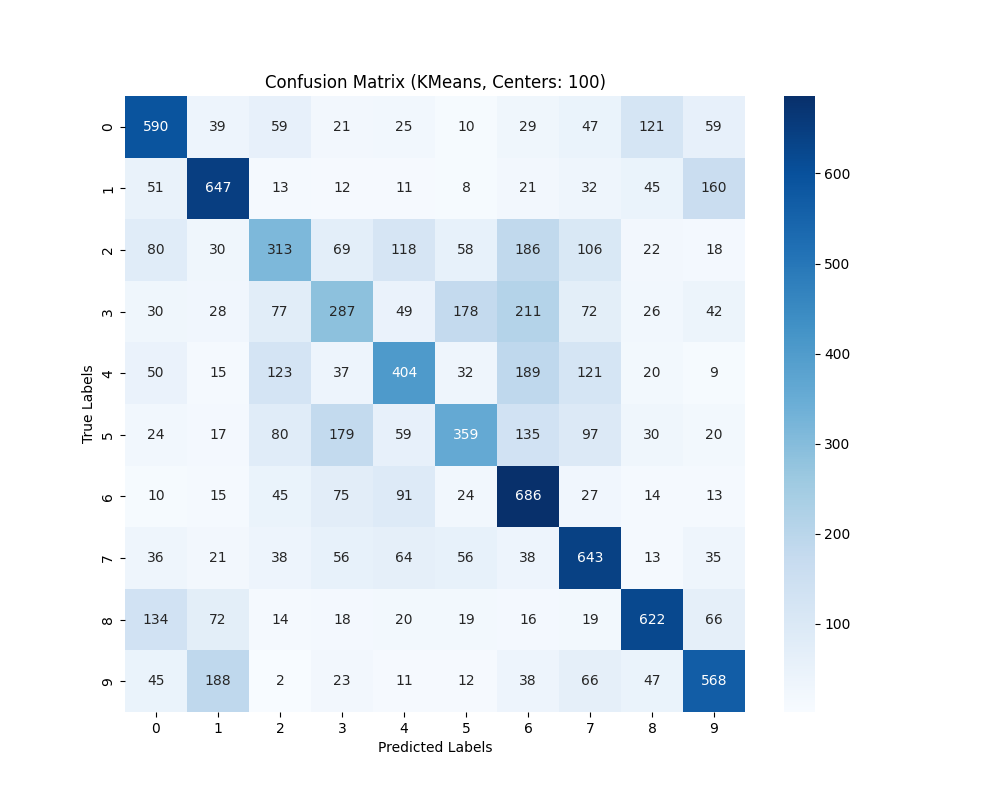
\includegraphics[width=0.48\textwidth]{confusion_matrix_KMeans_100.png}
    \caption{Confusion Matrix for KMeans initialization (100 Centers).}
    \label{fig:confusion-matrix-KMeans100}
\end{figure}

\begin{figure}[H]
    \centering
    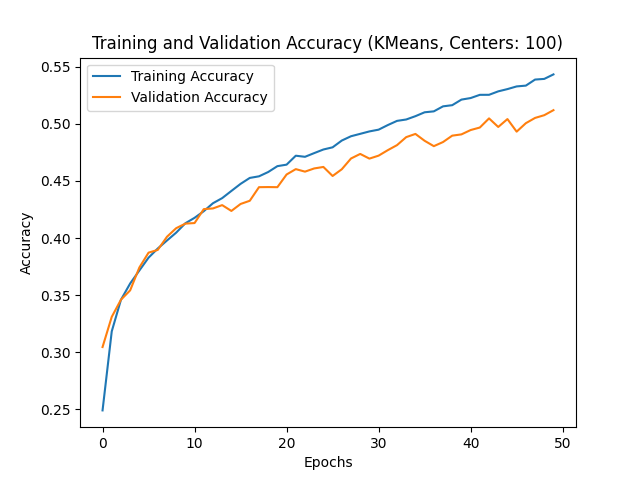
\includegraphics[width=0.48\textwidth]{training_validation_accuracy_KMeans_100.png}
    \caption{Training and Validation accuracy throughout epochs KMeans initialization (100 Centers).}
    \label{fig:TR100Centers}
\end{figure}

\begin{figure}[H]
    \centering
    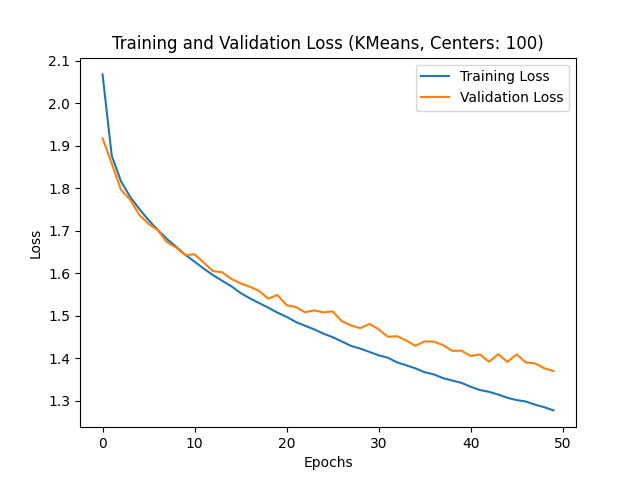
\includegraphics[width=0.48\textwidth]{training_validation_loss_KMeans_100.png}
    \caption{Training and Validation loss throughout epochs KMeans initialization (100 Centers).}
    \label{fig:TR100Centersloss}
\end{figure}

\begin{figure}[H]
    \centering
    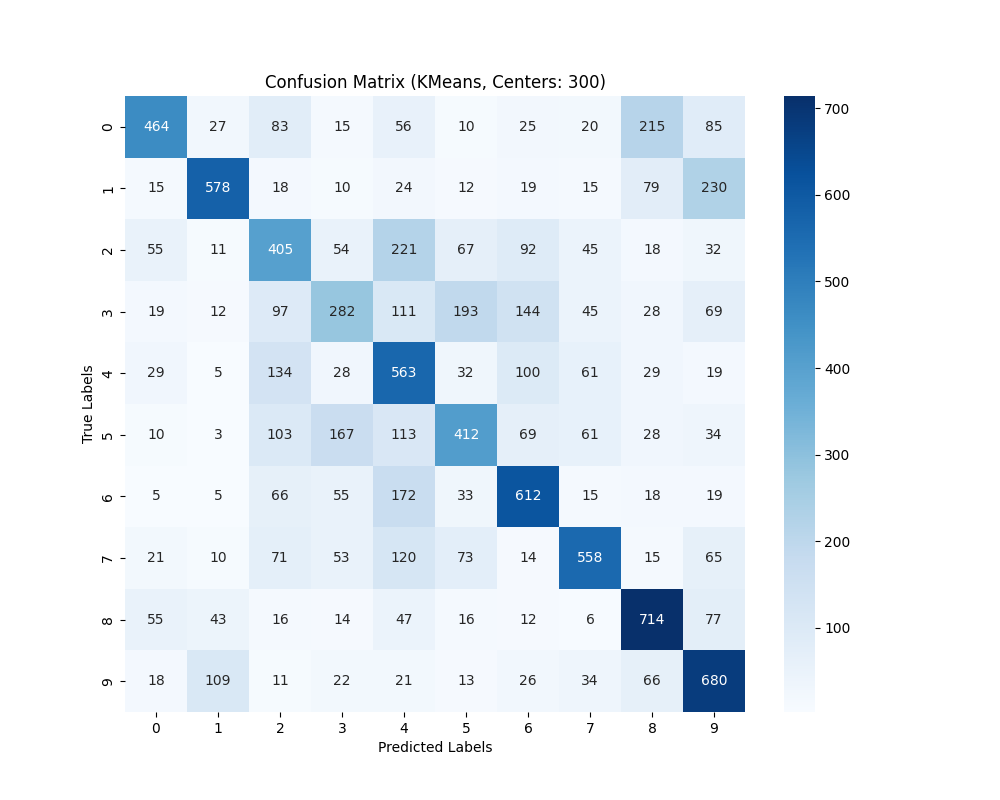
\includegraphics[width=0.48\textwidth]{confusion_matrix_KMeans_300.png}
    \caption{Confusion Matrix for KMeans initialization (300 Centers).}
    \label{fig:confusion-matrix-KMeans300}
\end{figure}

\begin{figure}[H]
    \centering
    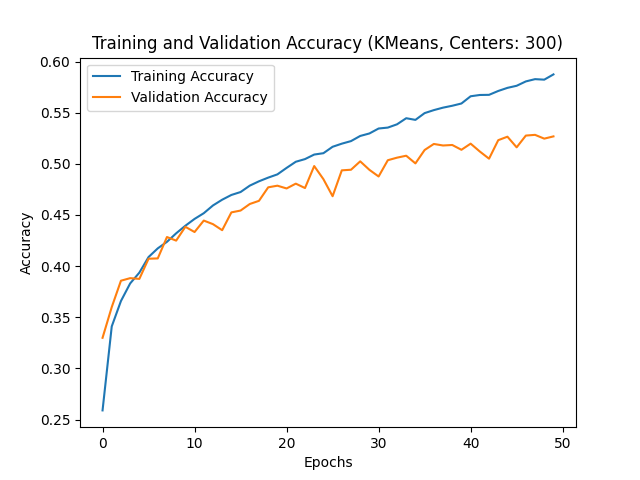
\includegraphics[width=0.48\textwidth]{training_validation_accuracy_KMeans_300.png}
    \caption{Training and Validation accuracy throughout epochs KMeans initialization (300 Centers).}
    \label{fig:TR300Centers}
\end{figure}

\begin{figure}[H]
    \centering
    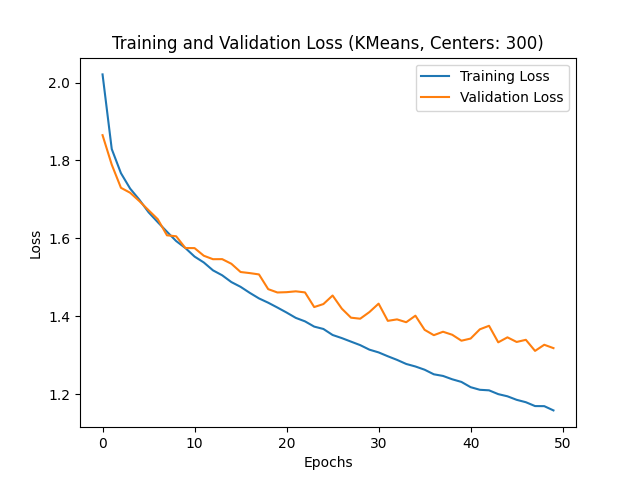
\includegraphics[width=0.48\textwidth]{training_validation_loss_KMeans_300.png}
    \caption{Training and Validation loss throughout epochs KMeans initialization (300 Centers).}
    \label{fig:TR300Centersloss}
\end{figure}

\begin{figure}[H]
    \centering
    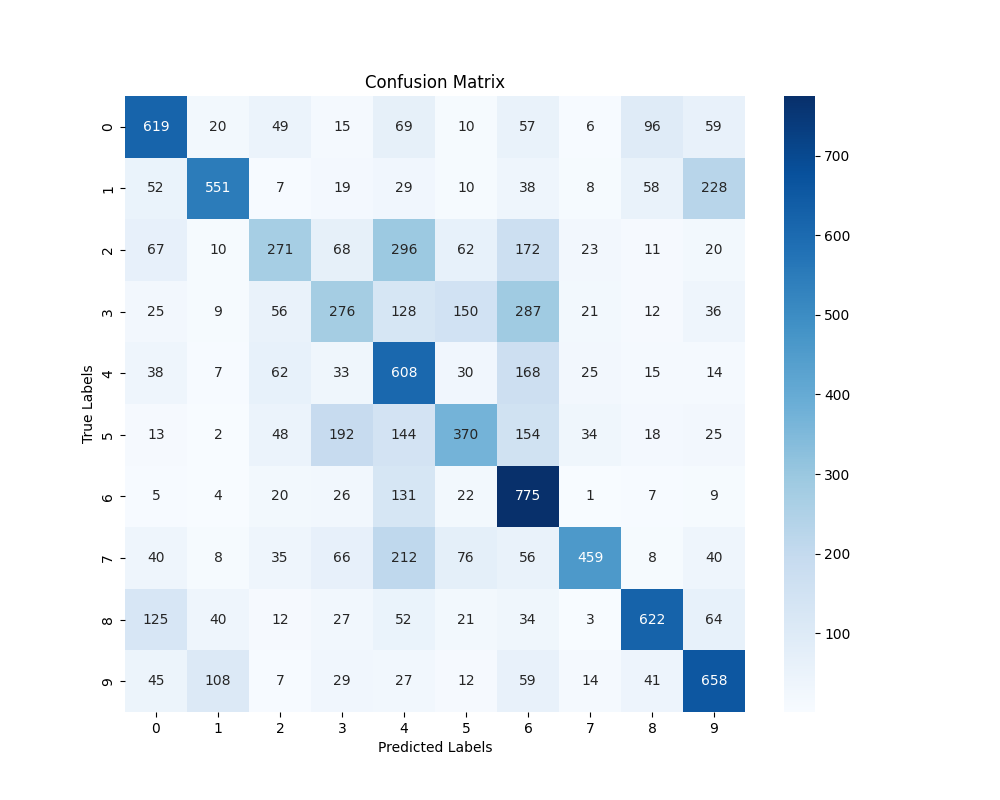
\includegraphics[width=0.48\textwidth]{confusion_matrix_KMeans_500.png}
    \caption{Confusion Matrix for KMeans initialization (500 Centers).}
    \label{fig:confusion-matrix-KMeans500}
\end{figure}

\begin{figure}[H]
    \centering
    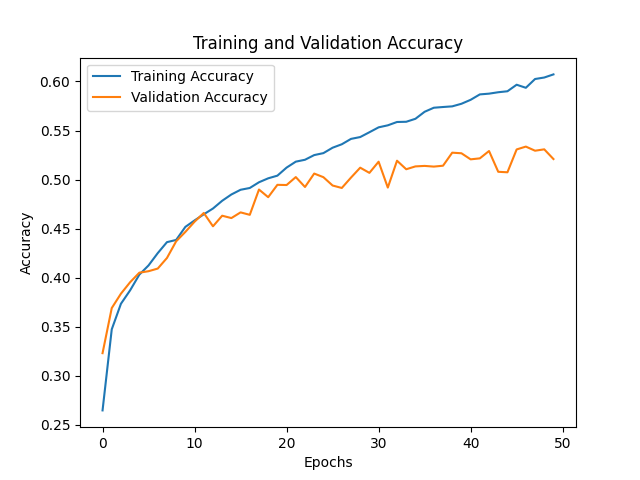
\includegraphics[width=0.48\textwidth]{training_validation_accuracy_KMeans_500.png}
    \caption{Training and Validation accuracy throughout epochs KMeans initialization (500 Centers).}
    \label{fig:TR500Centers}
\end{figure}

\begin{figure}[H]
    \centering
    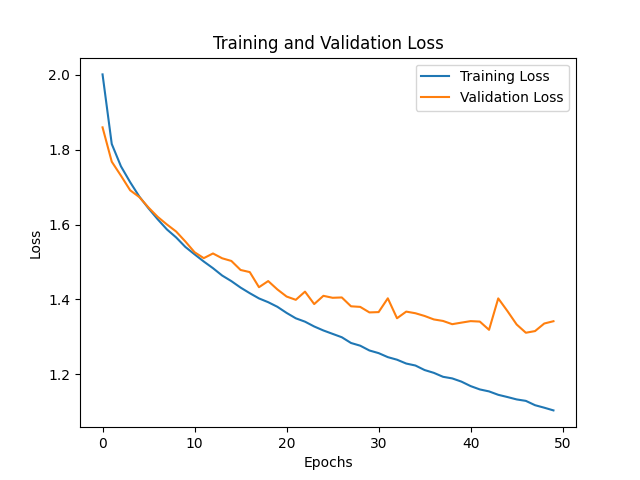
\includegraphics[width=0.48\textwidth]{training_validation_loss_KMeans_500.png}
    \caption{Training and Validation loss throughout epochs KMeans initialization (500 Centers).}
    \label{fig:TR500Centersloss}
\end{figure}

\begin{figure}[H]
    \centering
    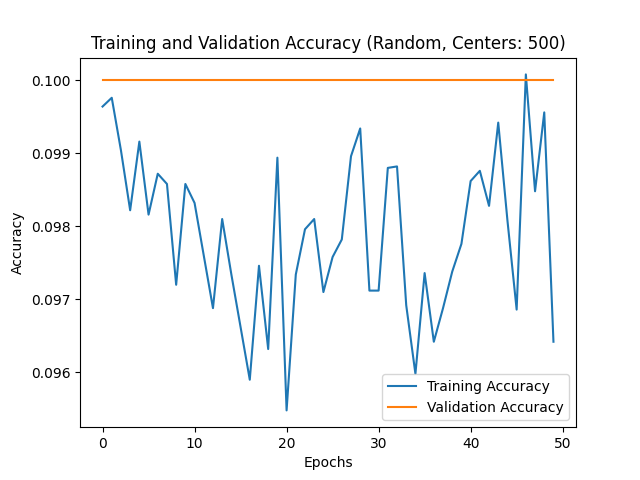
\includegraphics[width=0.48\textwidth]{training_validation_accuracy_Random_500.png}
    \caption{Training and Validation accuracy throughout epochs RANDOM initialization (500 Centers).}
    \label{fig:TR500RandCenters}
\end{figure}

The code corresponding to this initial implementation is in the \texttt{RBF\_gradientdescent.py} file.

\section{\textbf{Process for Comparative Experimentation with RBF Network and Other Classifiers}}

In this section, I detail the process followed to implement and evaluate the Radial Basis Function (RBF) network, k-Nearest Neighbors (k-NN), and Nearest Centroid classifiers as part of a comparative study on the CIFAR-10 dataset. The steps below describe how the tasks were carried out and the methodologies used.

\subsection{\textbf{Data Preparation and Dimensionality Reduction}}
\begin{itemize}
    \item \textbf{Dataset:} The CIFAR-10 dataset was loaded using a custom function \texttt{load\_cifar10\_data}, and it consists of 60,000 images classified into 10 categories. The images were flattened to vectors for further processing.
    \item \textbf{Principal Component Analysis (PCA):} To reduce the computational burden and extract meaningful features, PCA was applied to reduce the dimensionality of the data while retaining 90\% of the variance.
    \item The reduced-dimension data was then used as input for the RBF network, k-NN classifier, and Nearest Centroid classifier.
\end{itemize}

\subsection{\textbf{Implementation of the RBF Network}}
\begin{itemize}
    \item \textbf{Network Structure:} 
    The RBF network was implemented with a custom class, where the number of RBF centers (\texttt{num\_centers}) and the output dimensions (\texttt{output\_dim}) were defined as key hyperparameters.
    \item \textbf{Centers Initialization:} 
    KMeans clustering was used to initialize the centers of the RBF units. The calculated cluster centroids represent the RBF centers, ensuring optimal placement.
    \item \textbf{Sigma Calculation:} 
    The width parameter (\texttt{sigma}) of the RBF units was computed as the mean of the pairwise Euclidean distances between centers.
    \item \textbf{Interpolation Matrix:} 
    A Gaussian RBF function was applied to calculate the interpolation matrix, which maps input data to the RBF space.
    \item \textbf{Weights Computation:} 
    The network weights were computed using the inverse of the interpolation matrix and the one-hot encoded labels.
    \item \textbf{Training and Prediction:} 
    Training involved computing weights, while prediction used the interpolation matrix to calculate output probabilities. Accuracy and confusion matrices were recorded for evaluation.
\end{itemize}

\subsection{\textbf{Implementation of k-NN and Nearest Centroid Classifiers}}
\begin{itemize}
    \item \textbf{k-NN Classifier:}
    The k-NN classifier was implemented with different values of $k$ (1, 3, and 5). The classifier was trained on the PCA-reduced data, and predictions were made on the test set. Metrics such as training time, testing time, accuracy, confusion matrices, and classification reports were recorded for each $k$.
    \item \textbf{Nearest Centroid Classifier:}
    The Nearest Centroid classifier was implemented to classify samples based on the closest class centroid in the feature space. Similar metrics as the k-NN classifier were computed for evaluation.
\end{itemize}

\subsection{\textbf{Results of Various Classifiers}}

This section provides a comparative analysis of the performance of different classifiers: the RBF Network, k-Nearest Neighbors (k-NN), and the Nearest Centroid Classifier. Key metrics such as training time, testing time, accuracy, confusion matrices, and classification reports are summarized below.

\subsubsection{\textbf{RBF Network Results}}
\begin{itemize}
    \item \textbf{Training Time:} 18.05 seconds
    \item \textbf{Testing Time:} 3.24 seconds
    \item \textbf{Accuracy:} 41.45\%
\end{itemize}

\textbf{Confusion Matrix:}
\begin{scriptsize}
\[
\begin{bmatrix}
442 & 51 & 51 & 12 & 25 & 14 & 38 & 43 & 267 & 57 \\
29 & 497 & 16 & 26 & 15 & 16 & 60 & 46 & 108 & 187 \\
113 & 47 & 243 & 73 & 138 & 73 & 158 & 73 & 49 & 33 \\
59 & 75 & 59 & 227 & 55 & 181 & 148 & 83 & 38 & 75 \\
55 & 45 & 119 & 42 & 318 & 45 & 205 & 102 & 42 & 27 \\
31 & 51 & 86 & 150 & 61 & 327 & 120 & 99 & 43 & 32 \\
18 & 65 & 72 & 57 & 88 & 54 & 552 & 44 & 11 & 39 \\
41 & 57 & 37 & 50 & 118 & 57 & 77 & 419 & 40 & 104 \\
70 & 82 & 8 & 24 & 15 & 29 & 18 & 35 & 622 & 97 \\
40 & 193 & 10 & 17 & 10 & 17 & 50 & 53 & 112 & 498 \\
\end{bmatrix}
\]
\end{scriptsize}

\textbf{Classification Report:}
\begin{scriptsize}
\begin{verbatim}
              precision    recall  f1-score   support
           0       0.49      0.44      0.47      1000
           1       0.43      0.50      0.46      1000
           2       0.35      0.24      0.29      1000
           3       0.33      0.23      0.27      1000
           4       0.38      0.32      0.35      1000
           5       0.40      0.33      0.36      1000
           6       0.39      0.55      0.46      1000
           7       0.42      0.42      0.42      1000
           8       0.47      0.62      0.53      1000
           9       0.43      0.50      0.46      1000

    accuracy                           0.41     10000
   macro avg       0.41      0.41      0.41     10000
weighted avg       0.41      0.41      0.41     10000
\end{verbatim}
\end{scriptsize}

\subsubsection{\textbf{k-NN Classifier Results}}
The k-NN classifier was evaluated with three values of $k$: 1, 3, and 5. Below are the results:

\textbf{k = 1:}
\begin{itemize}
    \item \textbf{Training Time:} 0.04 seconds
    \item \textbf{Testing Time:} 1.67 seconds
    \item \textbf{Accuracy:} 38.58\%
\end{itemize}

\textbf{k = 3:}
\begin{itemize}
    \item \textbf{Training Time:} 0.01 seconds
    \item \textbf{Testing Time:} 1.52 seconds
    \item \textbf{Accuracy:} 36.59\%
\end{itemize}

\textbf{k = 5:}
\begin{itemize}
    \item \textbf{Training Time:} 0.01 seconds
    \item \textbf{Testing Time:} 1.37 seconds
    \item \textbf{Accuracy:} 38.07\%
\end{itemize}

\subsubsection{\textbf{Nearest Centroid Classifier Results}}
\begin{itemize}
    \item \textbf{Training Time:} 0.06 seconds
    \item \textbf{Testing Time:} 0.00 seconds
    \item \textbf{Accuracy:} 27.66\%
\end{itemize}

\textbf{Classification Report:}
\begin{scriptsize}
\begin{verbatim}
              precision    recall  f1-score   support
           0       0.27      0.54      0.36      1000
           1       0.28      0.19      0.22      1000
           2       0.28      0.11      0.16      1000
           3       0.26      0.06      0.09      1000
           4       0.27      0.12      0.16      1000
           5       0.27      0.29      0.28      1000
           6       0.22      0.54      0.31      1000
           7       0.26      0.16      0.20      1000
           8       0.42      0.37      0.39      1000
           9       0.33      0.41      0.36      1000

    accuracy                           0.28     10000
   macro avg       0.29      0.28      0.25     10000
weighted avg       0.29      0.28      0.25     10000
\end{verbatim}
\end{scriptsize}

\subsubsection{\textbf{Key Observations}}
\begin{itemize}
    \item The RBF Network outperformed other methods in terms of accuracy (41.45\%) but required significantly more training time than k-NN and Nearest Centroid classifiers.
    \item Among the k-NN configurations, $k=1$ provided the best accuracy (38.58\%), but its results were closer to random guessing compared to the RBF Network.
    \item The Nearest Centroid classifier had the fastest training and testing times but achieved the lowest accuracy (27.66\%).
    \item These results highlight the trade-off between computational efficiency and model accuracy.
\end{itemize}

\subsection{\textbf{Visualizations and Outputs}}
Below are visualizations of the confusion matrices and metrics for all classifiers:
\begin{figure}[H]
    \centering
    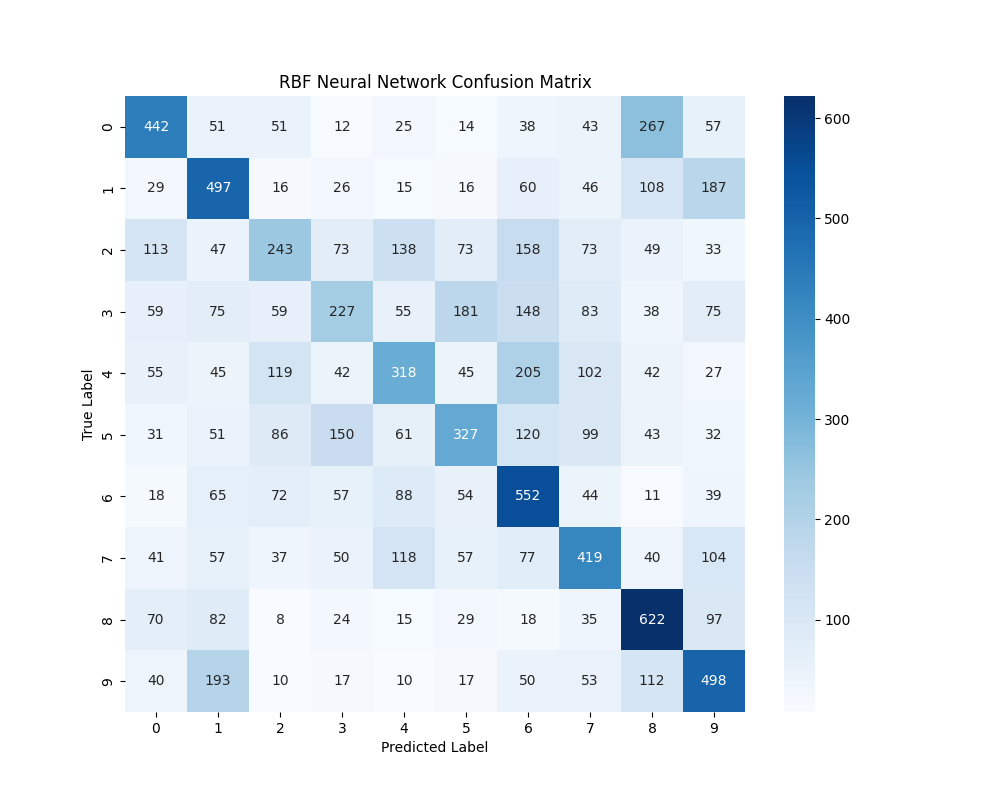
\includegraphics[width=0.48\textwidth]{conf_matrix_rbf.png}
    \caption{Confusion Matrix for RBF Network.}
    \label{fig:conf-matrix-rbf}
\end{figure}

\begin{figure}[H]
    \centering
    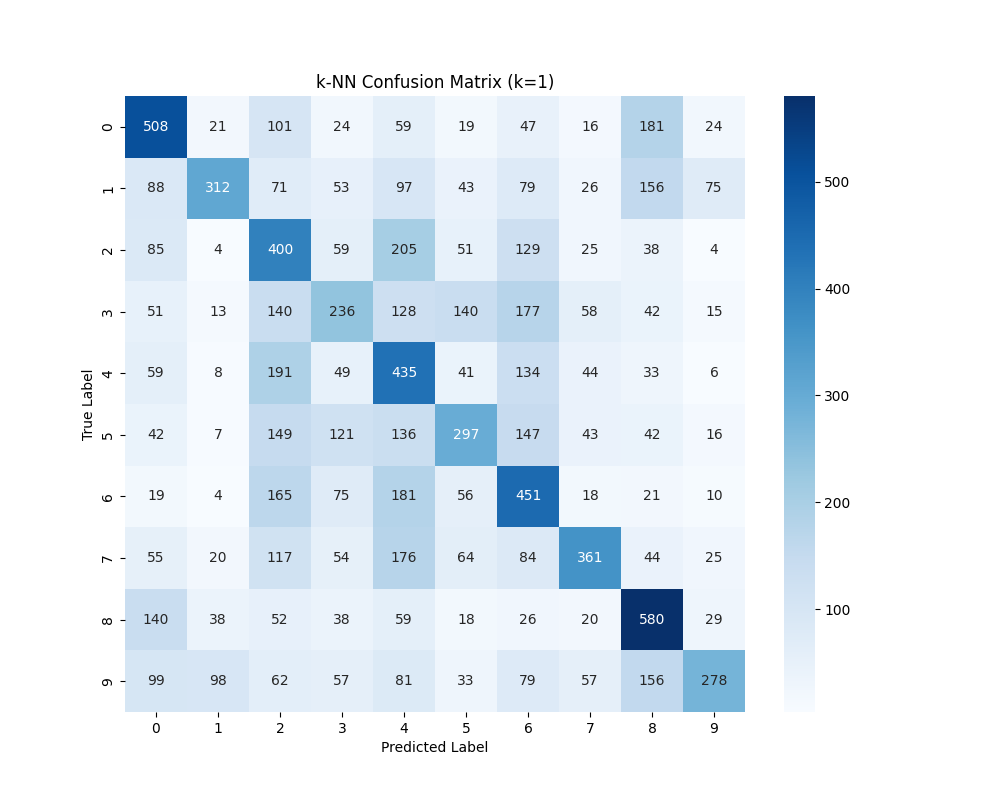
\includegraphics[width=0.48\textwidth]{conf_matrix_knn_k1.png}
    \caption{Confusion Matrix for k-NN Classifier ($k=1$).}
    \label{fig:conf-matrix-knn1}
\end{figure}

\begin{figure}[H]
    \centering
    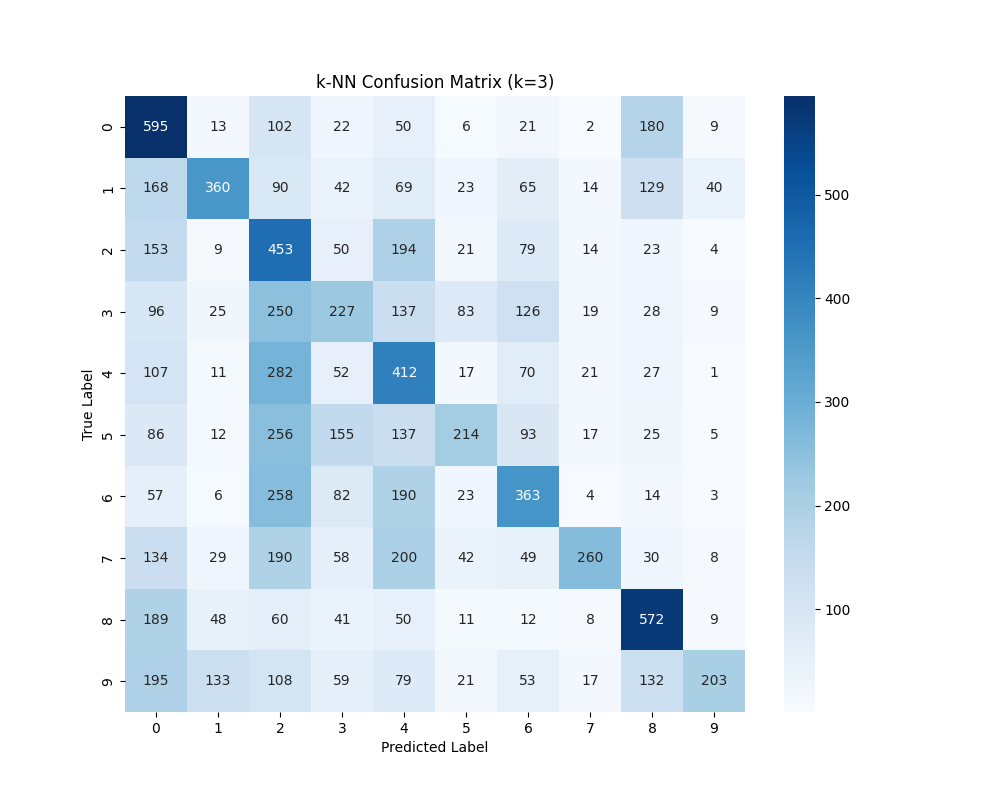
\includegraphics[width=0.48\textwidth]{conf_matrix_knn_k3.png}
    \caption{Confusion Matrix for k-NN Classifier ($k=3$).}
    \label{fig:conf-matrix-knn3}
\end{figure}

\begin{figure}[H]
    \centering
    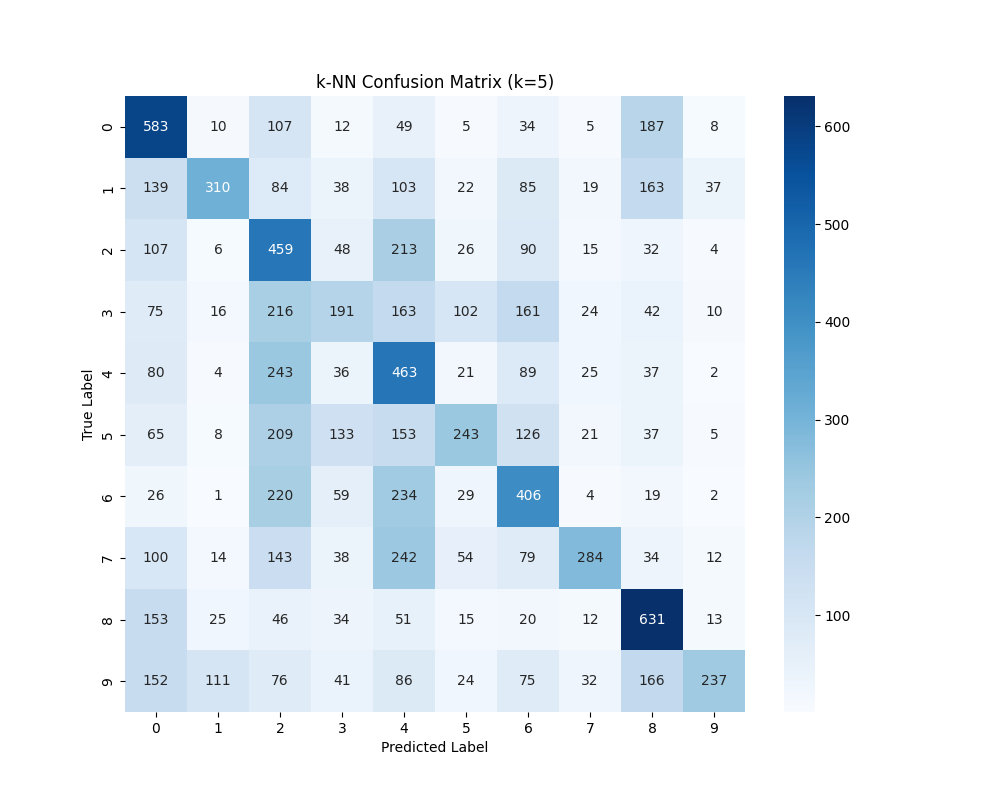
\includegraphics[width=0.48\textwidth]{conf_matrix_knn_k5.png}
    \caption{Confusion Matrix for k-NN Classifier ($k=5$).}
    \label{fig:conf-matrix-knn5}
\end{figure}

\begin{figure}[H]
    \centering
    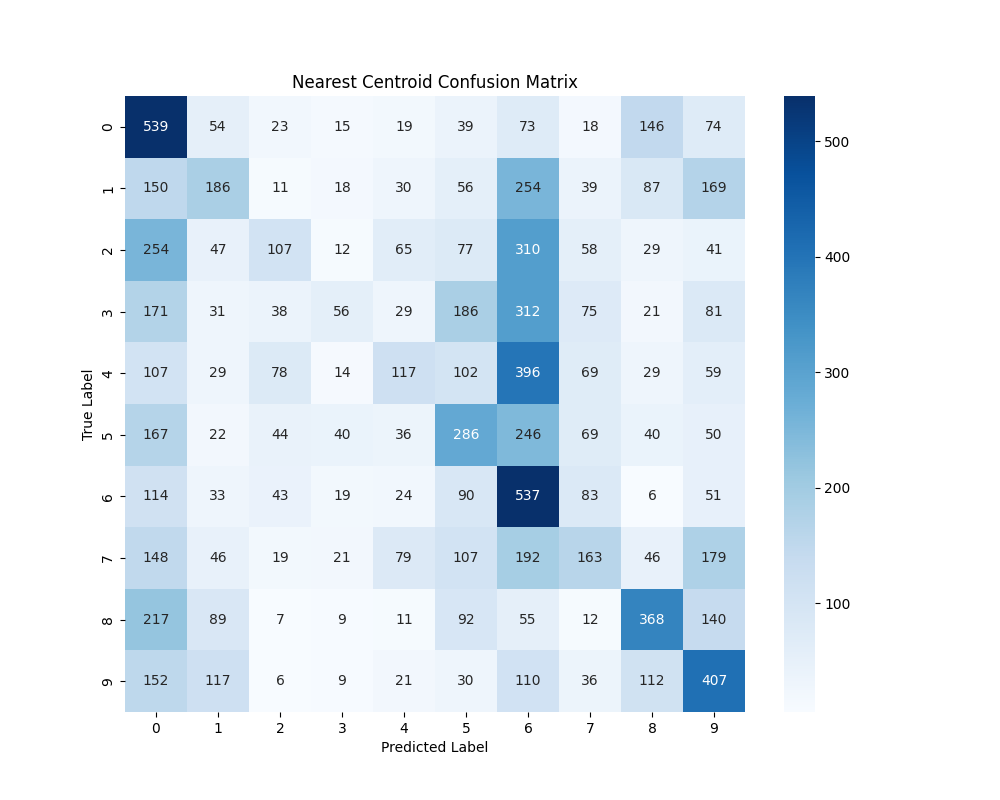
\includegraphics[width=0.48\textwidth]{conf_matrix_centroid.png}
    \caption{Confusion Matrix for Nearest Centroid Classifier.}
    \label{fig:conf-matrix-centroid}
\end{figure}

The code corresponding to this RBFN implementation is in the \texttt{rbf\_all.py} file.

\subsection{\textbf{An improved version of RBFN (experiment) ...}}
In this experiment, an improved version of the Radial Basis Function Network (RBFN) was implemented to address the limitations of the previous model. Key enhancements include the incorporation of adaptive sigmas for the RBF kernels, regularization to stabilize weight calculations, and batch-wise kernel computations for memory efficiency. The CIFAR-10 dataset was used to evaluate the model's performance.

\subsubsection{\textbf{Model Improvements}}
The following improvements were made to the RBFN:
\begin{itemize}
    \item \textbf{Adaptive Sigmas:} 
    - The sigma values for each RBF center were calculated based on the average distance to its nearest neighbors. This allows each RBF unit to adjust its width dynamically, improving the model's ability to capture local features in the data.
    \item \textbf{Regularization:} 
    - A small regularization term was added to the weights calculation to prevent overfitting and numerical instability during matrix inversion.
    \item \textbf{Batch-wise Kernel Computation:} 
    - To handle the high-dimensional CIFAR-10 data efficiently, the kernel matrix was computed in batches, reducing memory consumption and ensuring scalability.
\end{itemize}

\subsubsection{\textbf{Results}}
The improved RBFN was evaluated on the CIFAR-10 dataset, with the following results:

\begin{itemize}
    \item \textbf{Accuracy:} 47.19\%
    \item \textbf{Confusion Matrix:}
\end{itemize}

\begin{scriptsize}
\[
\begin{bmatrix}
528 & 47 & 54 & 14 & 23 & 7 & 34 & 44 & 189 & 60 \\
27 & 606 & 12 & 29 & 10 & 22 & 27 & 35 & 78 & 154 \\
92 & 50 & 302 & 79 & 128 & 58 & 150 & 78 & 35 & 28 \\
45 & 46 & 69 & 288 & 64 & 154 & 150 & 73 & 41 & 70 \\
56 & 37 & 142 & 43 & 361 & 36 & 167 & 102 & 36 & 20 \\
24 & 42 & 74 & 181 & 48 & 344 & 110 & 103 & 37 & 37 \\
9 & 33 & 63 & 59 & 101 & 41 & 609 & 39 & 22 & 24 \\
34 & 50 & 32 & 58 & 85 & 58 & 50 & 506 & 31 & 96 \\
80 & 85 & 14 & 29 & 14 & 19 & 14 & 22 & 646 & 77 \\
40 & 205 & 10 & 24 & 8 & 20 & 37 & 38 & 89 & 529 \\
\end{bmatrix}
\]
\end{scriptsize}

\textbf{Classification Report:}
\begin{scriptsize}
\begin{verbatim}
              precision    recall  f1-score   support
           0       0.56      0.53      0.55      1000
           1       0.50      0.61      0.55      1000
           2       0.39      0.30      0.34      1000
           3       0.36      0.29      0.32      1000
           4       0.43      0.36      0.39      1000
           5       0.45      0.34      0.39      1000
           6       0.45      0.61      0.52      1000
           7       0.49      0.51      0.50      1000
           8       0.54      0.65      0.59      1000
           9       0.48      0.53      0.51      1000
    accuracy                           0.47     10000
   macro avg       0.47      0.47      0.46     10000
weighted avg       0.47      0.47      0.46     10000
\end{verbatim}
\end{scriptsize}

\subsubsection{\textbf{Key Observations}}
\begin{itemize}
    \item The improved RBFN achieved an accuracy of 47.19\%, which is higher than the traditional RBFN (41.45\%). This demonstrates the effectiveness of adaptive sigmas and regularization.
    \item The confusion matrix shows better class separation compared to the previous implementation, though certain classes (e.g., 3 and 5) still exhibit significant confusion.
    \item The classification report highlights that precision and recall values are fairly balanced across classes, with higher scores for simpler classes like 0 and 8.
    \item The improved RBFN remains computationally efficient due to the use of batch-wise kernel computation.
\end{itemize}

\subsubsection{\textbf{Visualizations}}
The following visualizations illustrate the performance of the improved RBFN:

\begin{figure}[H]
    \centering
    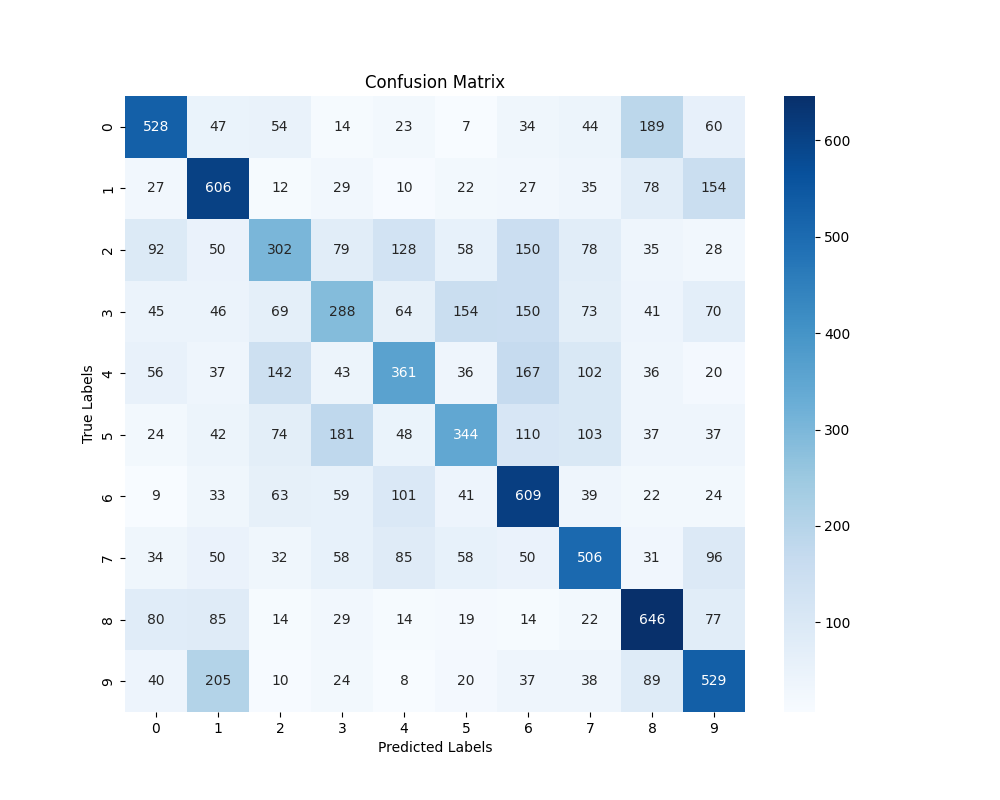
\includegraphics[width=0.48\textwidth]{improved_confusion_matrix.png}
    \caption{Confusion Matrix for the Improved RBFN.}
    \label{fig:improved-confusion-matrix}
\end{figure}

\subsubsection{\textbf{Summary}}
The improved RBFN shows significant gains over the basic RBFN by taking advantage of adaptive sigmas, regularization, and batch-wise computations. These additions resulted in better class separability, improved accuracy, and efficient training. 

The code corresponding to this improved implementation is in the \texttt{RBF\_improved.py} file.

\subsection{\textbf{Summary of Observations}}
\begin{itemize}
    \item The RBF network performed well but required significant computational resources for training compared to the other classifiers.
    \item The k-NN classifier achieved the highest accuracy, but its testing time increased with the dataset size.
    \item The Nearest Centroid classifier was the fastest and simplest to implement but lagged slightly in accuracy compared to the k-NN classifier.
    \item The choice of classifier depends on the trade-off between accuracy and computational efficiency for the given application.
    \item \textbf{\textbf{It is very very important}} to note from this experiment that the trainable RBF Neural Network (RBFNN) implemented in the previous sector performed better than the Radial Basis Function Network (RBFN) (even the attempt for an improved version) where the weights were computed using the inverse of the interpolation matrix rather than with backpropagation and gradient-based optimization and sigmas are not trainable. This result highlights the advantage of allowing trainable centers and weights, which enable the model to better adapt to the dataset through iterative optimization. In contrast, the fixed-weight RBFN's reliance on analytical solutions, while computationally simpler, limits its capacity to learn complex patterns. Now I should also add here that the RBFNN I implemented in the previous sector outperforms the k-NN and Nearest Centroid Classifier as well, not only the RBF Network I showcased here.
\end{itemize}

\section{\textbf{Initial Autoencoder (MNIST)}}

This section explains how an autoencoder was used to reconstruct images from the MNIST dataset. An autoencoder is a model that compresses data into a smaller size and then learns to recreate the original data from this compressed version.

\subsection{\textbf{Model Design}}
The autoencoder has two main parts:
\begin{itemize}
    \item \textbf{Encoder:} 
    \begin{itemize}
        \item Shrinks the input image into a smaller, compressed form (latent space).
        \item Uses two layers of filters (convolutions) and pooling to extract features.
        \item Compresses the features into a 32-dimensional vector.
    \end{itemize}
    \item \textbf{Decoder:}
    \begin{itemize}
        \item Recreates the original image from the 32-dimensional vector.
        \item Uses layers that expand the size of the image step by step.
    \end{itemize}
\end{itemize}

\subsection{\textbf{How the Model was Trained}}
\begin{itemize}
    \item \textbf{Data:} 
    - The MNIST dataset contains 60,000 gray images of numbers (size $28 \times 28$).
    \item \textbf{Preprocessing:} 
    - The image pixel values were scaled to be between 0 and 1.
    \item \textbf{Training:}
    \begin{itemize}
        \item The model learned to match its outputs to the original images.
        \item It was trained for 15 rounds (epochs) with a batch size of 128 images at a time.
        \item A part of the data (20\%) was used for validation.
    \end{itemize}
\end{itemize}

\subsection{\textbf{Results}}
The autoencoder was able to recreate images from the MNIST dataset with high accuracy:
\begin{itemize}
    \item \textbf{Reconstruction Accuracy (1 - MSE):} 99.25\%
    \item \textbf{Training and Validation Loss:} 
    - Figure \ref{fig:training-loss} shows the error steadily reducing as the model improved.
    \item \textbf{Reconstructed Images:} 
    - Figure \ref{fig:autoencoder-results} compares the original and recreated images. The recreated images look almost the same as the originals.
\end{itemize}

\subsection{\textbf{Visualizations and Plots}}

\begin{figure}[H]
    \centering
    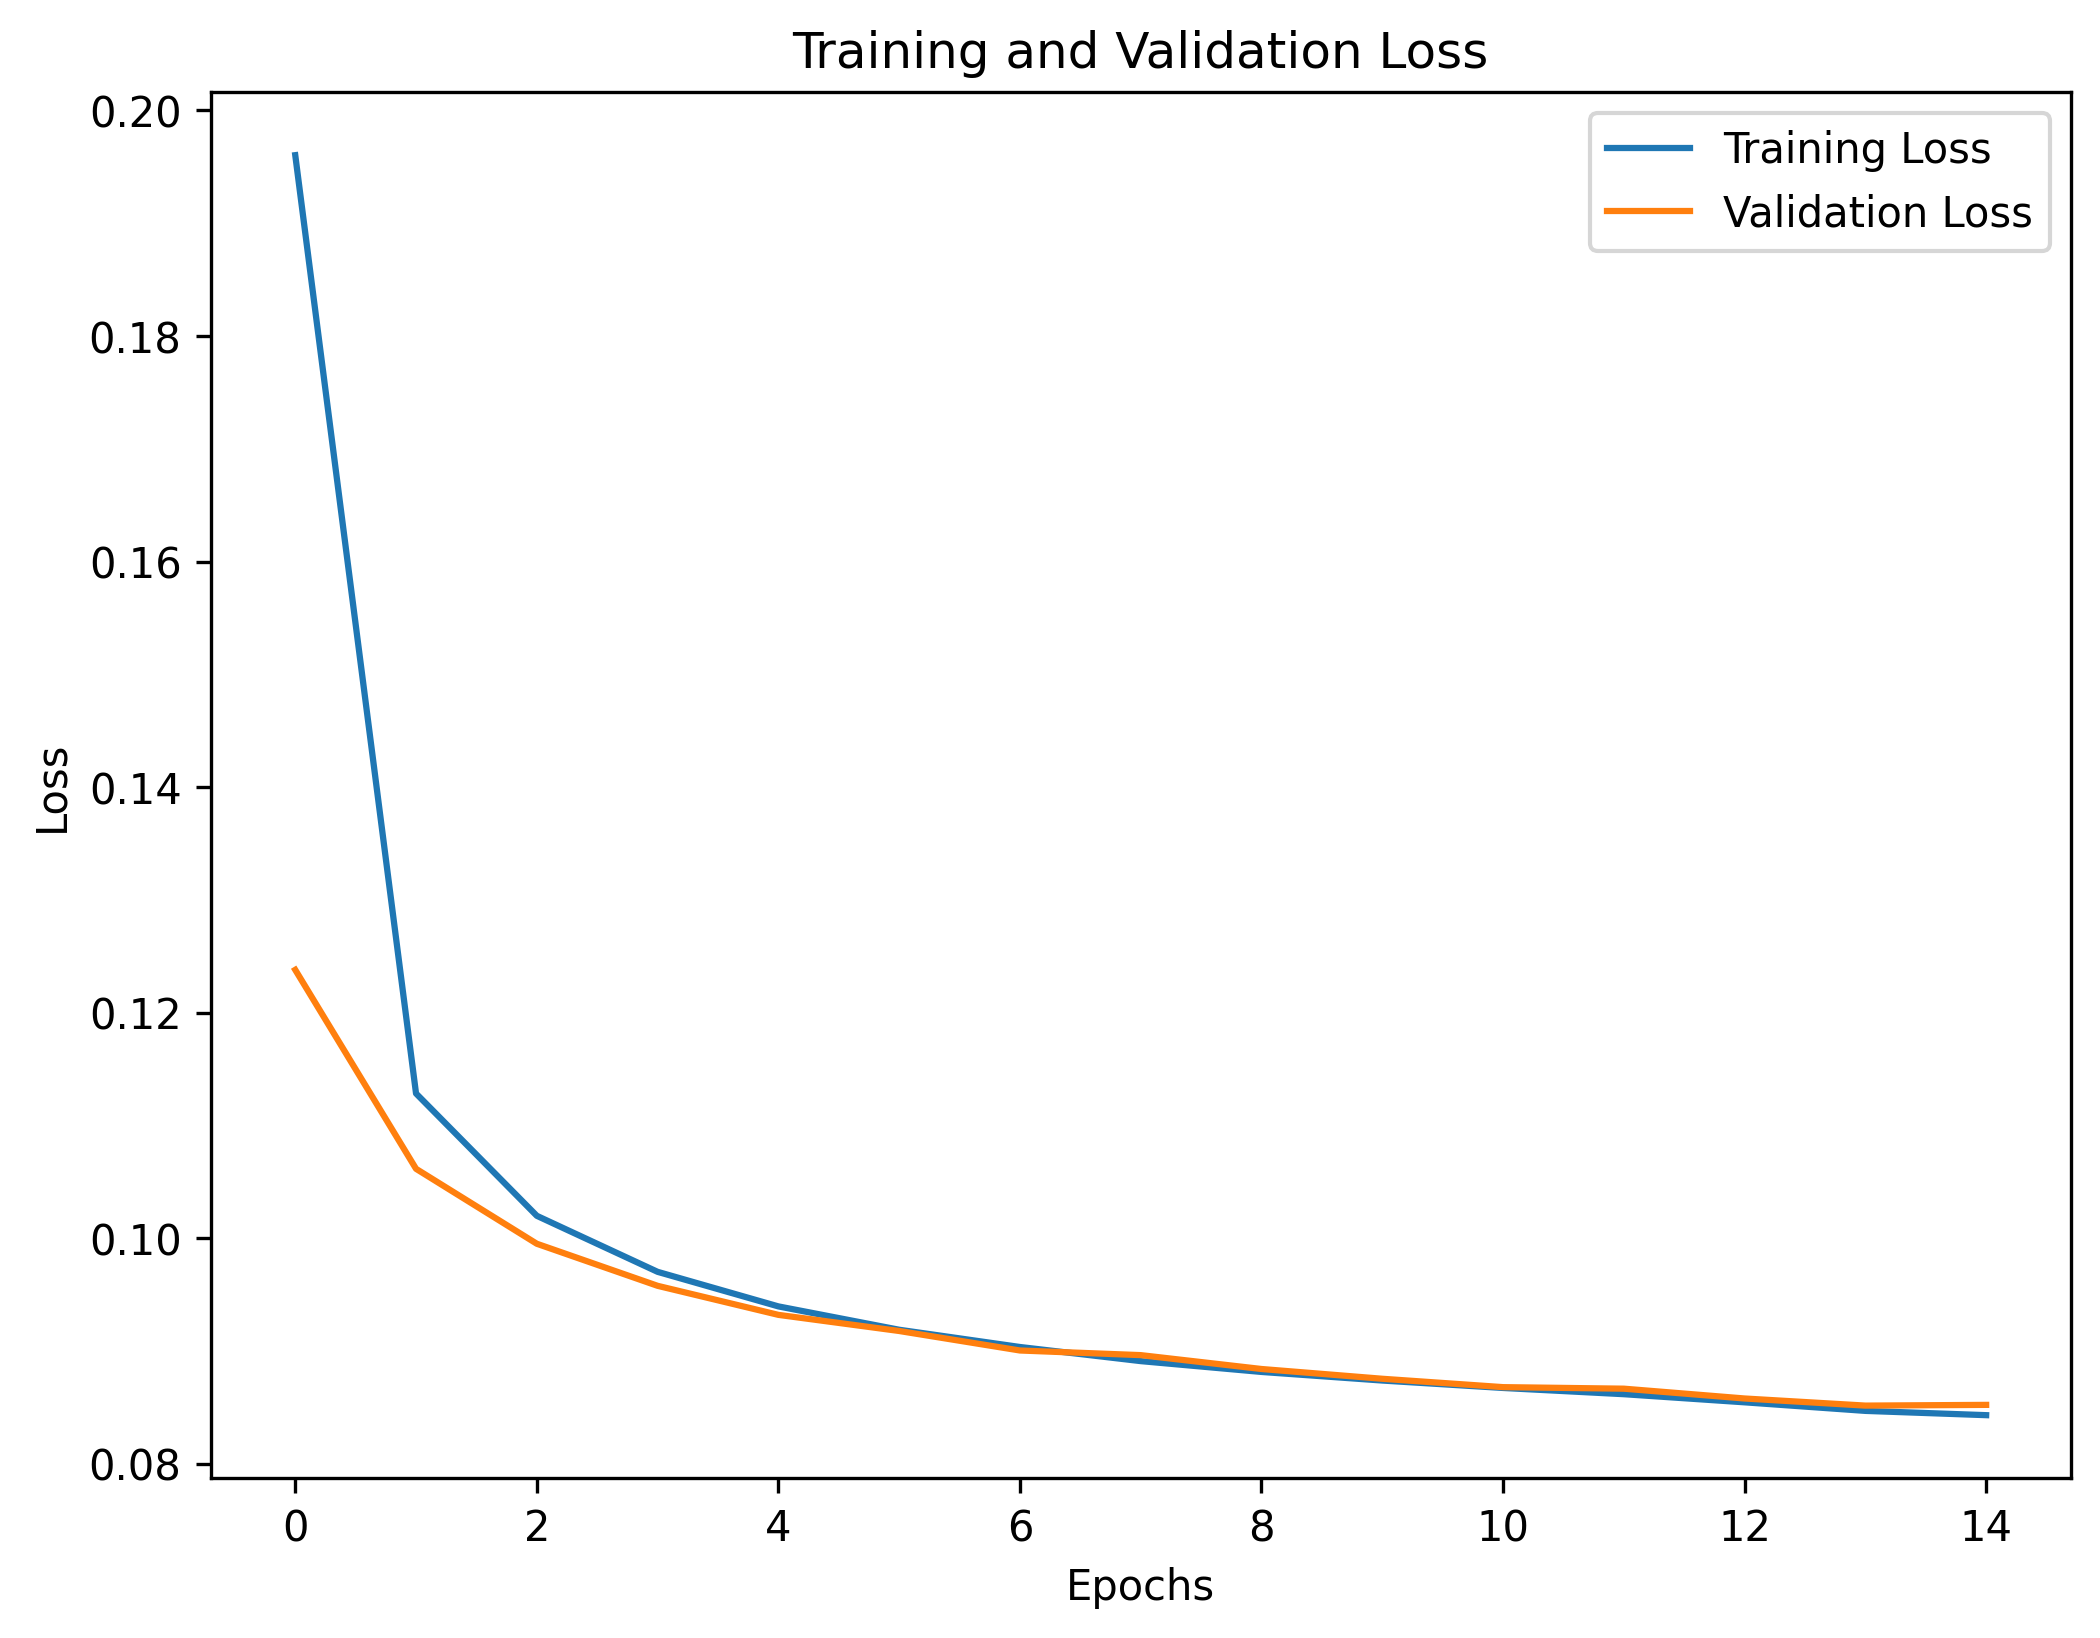
\includegraphics[width=0.48\textwidth]{mnist_training_loss.png}
    \caption{Training and Validation Loss for the Autoencoder on MNIST.}
    \label{fig:training-loss}
\end{figure}

\begin{figure}[H]
    \centering
    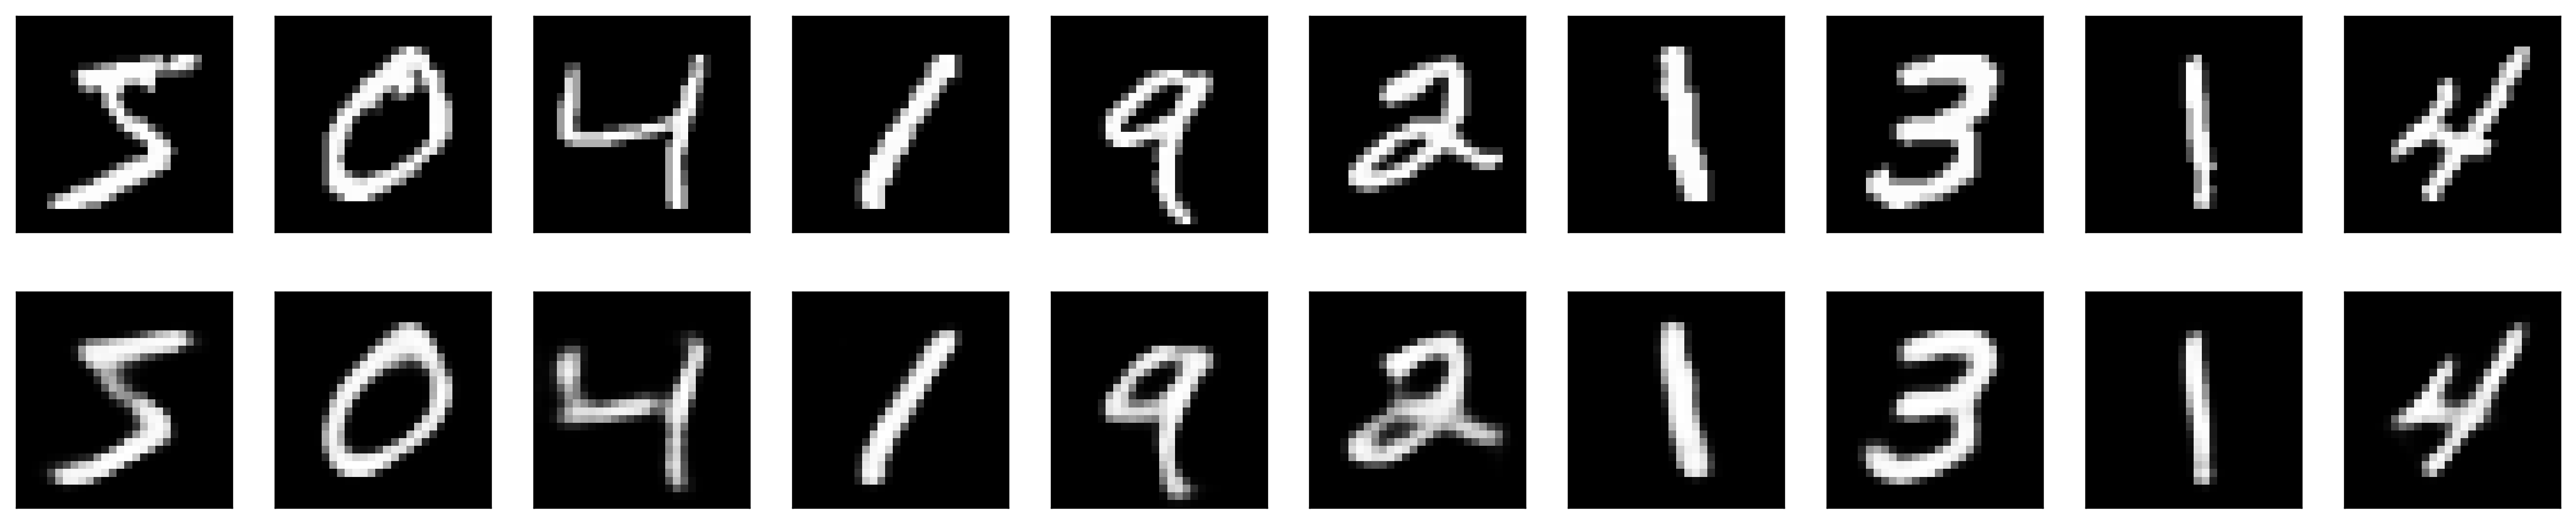
\includegraphics[width=0.48\textwidth]{autoencoder_results.png}
    \caption{Comparison of Original and Reconstructed Images. Top row: Original images. Bottom row: Reconstructed images. (MNIST)}
    \label{fig:autoencoder-results}
\end{figure}


\subsection{\textbf{What We Learned}}
\begin{itemize}
    \item The model did a great job at recreating images, with a very high reconstruction accuracy (99.25\%).
    \item The recreated images are very similar to the original ones, as seen in Figure \ref{fig:autoencoder-results}.
    \item The model’s error reduced steadily during training, as shown in Figure \ref{fig:training-loss}.
    \item This is a good first step in testing autoencoders. The simple MNIST data made it easier for the model to perform well.
\end{itemize}

\subsection{\textbf{Summary}}
This experiment showed that an autoencoder can effectively compress and recreate MNIST images. The model’s high accuracy and quality outputs make it a strong starting point for more advanced experiments, such as using harder datasets or adding new features like removing noise.

The code corresponding to this initial autoencoder for MNIST dataset implementation is in the \texttt{autoencoder\_mnist.py} file.

\section{\textbf{Autoencoder for CIFAR-10 (TensorFlow Implementation)}}

This section describes the use of an autoencoder to reconstruct images from the CIFAR-10 dataset. The autoencoder was built and trained using TensorFlow and evaluated for its ability to recreate the original images.

\subsection{\textbf{Model Design}}
The autoencoder has two main parts:
\begin{itemize}
    \item \textbf{Encoder:} 
    \begin{itemize}
        \item Compresses the input image into a smaller, simpler representation using two convolutional layers.
        \item Each layer reduces the size of the image while learning important features.
    \end{itemize}
    \item \textbf{Decoder:} 
    \begin{itemize}
        \item Recreates the original image from the compressed representation.
        \item Uses two transposed convolutional layers to restore the image size and details.
    \end{itemize}
\end{itemize}

\subsection{\textbf{Training Details}}
\begin{itemize}
    \item \textbf{Data:} 
    - CIFAR-10 dataset with 50,000 images was used for training.
    \item \textbf{Preprocessing:} 
    - Images were normalized so their pixel values ranged between 0 and 1.
    \item \textbf{Training Configuration:}
    \begin{itemize}
        \item Batch size: 64 images
        \item Number of epochs: 10
        \item Loss function: Mean squared error
        \item Optimizer: Adam with a learning rate of 0.001
    \end{itemize}
    \item \textbf{Output:}
    - You can find my results in the the file:
    \texttt{autoencoder\_results\_tf\_cifar.txt}.
\end{itemize}

\subsection{\textbf{Results}}
The autoencoder’s performance was evaluated by comparing the reconstructed images to the originals. The following results were obtained:
\begin{itemize}
    \item \textbf{Training Time:} 95.14 seconds
    \item \textbf{Final Training Loss:} 0.0013
    \item \textbf{Reconstruction Accuracy (1 - MSE):} 0.9988
\end{itemize}

\subsection{\textbf{Visualizations}}
The comparison between the original and reconstructed images is shown in Figure \ref{fig:comparison-tf-cifar}. The top row shows the original images, while the bottom row shows their reconstructions.

\begin{figure}[H]
    \centering
    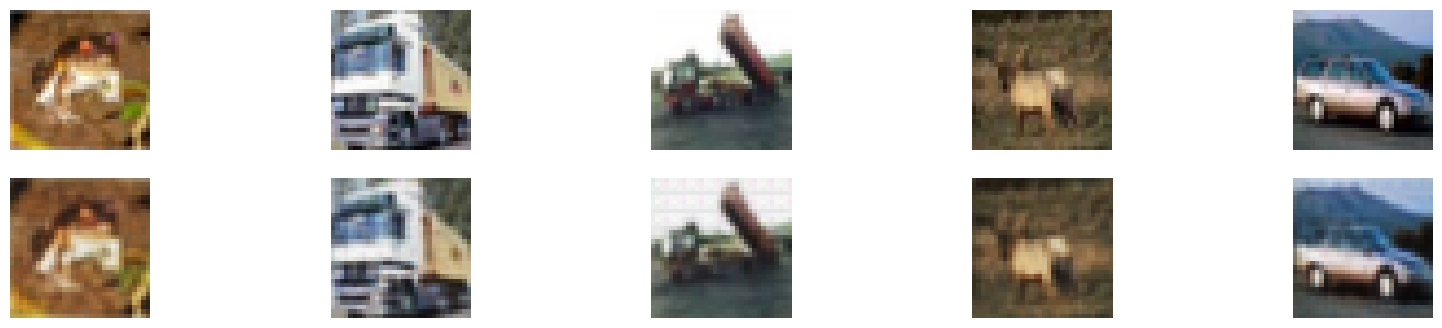
\includegraphics[width=0.48\textwidth]{autoencoder_comparison_tf_cifar.png}
    \caption{Comparison of Original and Reconstructed Images. Top row: Original images. Bottom row: Reconstructed images.}
    \label{fig:comparison-tf-cifar}
\end{figure}

\subsection{\textbf{What We Learned}}
\begin{itemize}
    \item The autoencoder performed exceptionally well, achieving a reconstruction accuracy of 99.88\%.
    \item The training process was efficient, taking only 95.14 seconds to complete 10 epochs, with a very low final loss of 0.0013.
    \item The reconstructed images are nearly identical to the original ones, as seen in Figure \ref{fig:comparison-tf-cifar}.
    \item This experiment demonstrates that a simple autoencoder architecture can handle the colorful and complex images in CIFAR-10 effectively.
\end{itemize}

\subsection{\textbf{Summary}}
The TensorFlow autoencoder successfully compressed and recreated CIFAR-10 images with extremely high accuracy. The results show that the model is highly efficient and a solid foundation for further experiments or extensions.

The code corresponding to this autoencoder for the Cifar10 dataset implementation is in the \texttt{autoencoder\_cifar10.py} file.

\section{\textbf{References Section}}
\begin{thebibliography}{1}
\bibliographystyle{IEEEtran}
\bibitem{ref1}
https://www.ibm.com/topics/knn
\bibitem{ref2}
https://en.wikipedia.org/wiki/Radial\_basis\_function\_kernel
\bibitem{ref3}
https://www.geeksforgeeks.org/auto-encoders/
\bibitem{ref5}
https://keras.io/api/datasets/mnist/
\bibitem{ref6}
https://www.cs.toronto.edu/~kriz/cifar.html
\bibitem{ref7}
https://en.wikipedia.org/wiki/Radial\_basis\_function\_network
\end{thebibliography}

\end{document}


